\section{MList}
Die \ac{MList} ist eine mehrstufige \ac{PQ}-Implementation, welche auf allen Ebenen \acp{LL} verwendet.

Die MList besteht aus drei Ebenen:
Die unterste Ebene (T3) ist eine �berschussliste f�r Elemente in entfernter Zukunft. Dies ist eine einfache \ac{LL} von Elementen.
Auf zweiter Ebene (T2) gibt es eine \ac{LL} von Buckets gleicher Breite. Die Buckets sind monoton fallend nach Priorit�ten sortiert ($ \forall x\in B_i,y \in B_{i+1}\colon x\leq y$). Die Elemente innerhalb eines Buckets sind unsortiert in einer \ac{LL} gespeichert.

Auf der h�chsten Ebene (T1) befinden sich die Elemente des aktuellen Buckets in einer sortierten \ac{LL}. \cite{li_mlist}

\begin{figure}[htb]
	\centering
	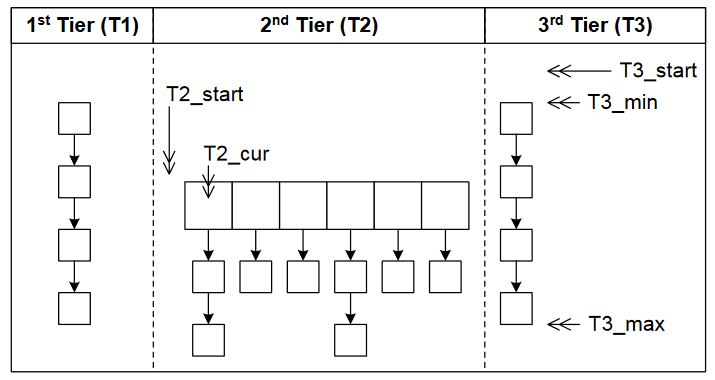
\includegraphics[width=0.4\textwidth]{images/mlist_structure}\caption{Struktur MList \cite{li_mlist}}\label{MList-struktur}
\end{figure}

In T2 wird \textit{\ac{bw}} wie folgt berechnet: 
\begin{equation}
	T2\_bw = \frac{T3\_max - T3\_min}{T3\_count}
\end{equation}

Die Ober- bzw. Untergrenze der Priorit�ten in T3 wird durch \textit{T3\_max} resp. \textit{T3\_min} gegeben; \textit{T3\_count} ist die Anzahl der Elemente in T3.
Die h�chste Priorit�t in T3 wird von \textit{T3\_start} angegeben. Analog dazu ist \textit{T2\_start} die h�chste Priorit�t aus T2.
Der aktuell kleinste nichtleere Bucket in T2 wird durch \textit{T2\_cur} markiert. Werden die Elemente eines Buckets nach T1 �berf�hrt, zeigt \textit{T2\_cur} auf den nachfolgen Bucket in T2.

\subsection{Dequeueing}
Initial ist ausschlie�lich T3 bef�llt. Beim ersten \textit{Dequeue} werden alle Elemente nach T2 verschoben und in Buckets eingeordnet. Anschlie�end werden die Elemente im ersten Bucket (bzw. \textit{T2\_cur}) sortiert und nach T1 verschoben. Ist in einem Bucket nur ein Element, braucht dieses nicht nach T1 verschoben werden, sondern kann direkt zur�ckgegeben werden.
Wenn T1 leer ist, wird der n�chste nicht leere Bucket nach T1 �berf�hrt. Wenn T2 leer ist, werden die zuvor benannten Schritte wiederholt. Das \ac{PES} ist leer, wenn alle Ebenen leer sind.

\subsection{Enqueueing}
Beim \textit{Enqueueing} wird durch die Ebenen T3 bis T1 durchgegangen, um den Einf�gepunkt zu ermitteln. Sobald dieser gefunden ist, kann abgebrochen werden.
F�llt das Element in den Bereich von T3, d.h. wenn es gr��er oder gleich \textit{T3\_start} ist, wird es an das Ende der \ac{LL} geh�ngt.
Andernfalls wird gepr�ft, ob die Priorit�t niedriger als \textit{T2\_cur} ist. Trifft dies zu, wird das Element in den Bucket mit Index \textit{bucket\_idx}, gem�� Gleichung \ref{MList-bucket-index} eingef�gt.
Falls dies nicht zutrifft, wird das Element in T1 einsortiert.\cite{li_mlist}


\begin{equation}
	bucket\_idx = \frac{priority - T2\_start}{T2\_bw}\label{MList-bucket-index}\hspace{1em}vgl. \cite{li_mlist}
\end{equation}

\subsection{Performance}
Die \ac{MList} ist so entworfen, dass bei jedem Sortiervorgang in T1 m�glichst wenige Elemente sortiert werden m�ssen.
Die amortisierte Zeit f�r das \textit{Dequeue} ist nach Li und Thng bei $O(1)$, da die Zeit f�r das Sortieren von wenigen Elementen vernachl�ssigbar ist. \cite{li_mlist}
Weil die \ac{LL} bei jeder �berf�hrung von T2 nach T1 sortiert werden muss, ist die theoretische Zeitkomplexit�t die des genutzten Sortieralgorithmus. 

Da in T2 die Elemente nur in Buckets eingeordnet werden, ist dies weniger aufwendig, als ein vollst�ndiger Sortiervorgang. \cite{li_mlist}
In \cite{bucket-sort} wird geschrieben, dass die Zeitkomplexit�t von \textit{Bucket Sort} bei $O(n)$ liegt. Jedoch auch, dass andere Algorithmen f�r besonders kleine oder besonders gro�e Listen �hnlich schnell oder schneller sind.

In T3 wird nicht sortiert, sondern immer am Ende angef�gt. Daraus ergibt sich $\Theta (1)$ f�r das Einf�gen auf dieser Ebene.

%\begin{figure}[htb]
%    \centering
%    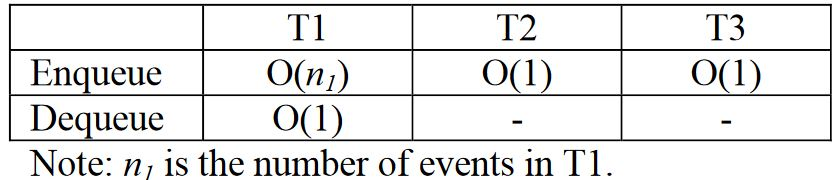
\includegraphics[width=0.7\textwidth]{images/mlist_complexity}\caption{Amortisierte Zeitkomplexit�t der MList Operationen \cite{li_mlist}}\label{MList-complexity}
%\end{figure}


Unter Verwendung von Alternativen zur \ac{LL} kann u.U. bei der �berf�hrung von einer Ebene in die n�chste ein Performancegewinn erzielt werden. \cite{exp-s-t}\cite{deterministic-sorting}